\chapter{Veje og Kredse}

\section{Veje}
Veje i en graf viser, hvilke ruter der er rundt i en graf. Dette er relevant for at finde ruter til en GPS, et computernetværk eller andet, hvor der er behov for at bestemme en rute gennem flere steder. 
En vej i en graf defineres i Definition \ref{def_vej}.

\begin{defn} \label{def_vej}
	Lad $n \in  \mathbb{Z}^{+}$ og lad $G$ være en ikke-orienteret graf. 
	En \textit{vej} af \textit{længde} $n$ fra $v_0$ til $v_n$ i $G$ er en sekvens af $n$ kanter $e_1, ..., e_n$ i $G$, for hvilke der eksisterer en sekvens $v_0,v_1,...,v_{n-1},v_n$ af knuder, så $e_i$ har endeknuderne $v_{i-1}$ og $v_i$ for $i=1,...,n$.
\end{defn}

Når der er tale om en vej gennem en simpel graf, angives denne som sekvensen af de knuder, den går igennem $v_0, v_1,...,v_n$. 
En vej er \textit{simpel} hvis den ikke indeholder den samme kant mere end én gang. 

\begin{exmp} \label{ex_vej}
	På den simple graf i Figur \ref{graf_vej} ses en simpel vej $A,B,E,F$ af længden 3, fordi vejen går gennem de tre kanter $\lbrace A,B \rbrace$, $\lbrace B,E \rbrace$ og $\lbrace E,F \rbrace$. 
	Vejen er simpel, fordi den ikke går gennem den samme kant mere end en gang. 
	Derimod er $A,B,D,E$ ikke en vej, fordi $\lbrace B,D \rbrace$ ikke er en kant. 
	Vejen $A,B,C,E,B,A$ er også en vej, men den er ikke simpel, fordi den går gennem kanten $\lbrace A,B \rbrace$ to gange. 
\end{exmp}

\begin{figure}[h]
	\centering
	\input{fig/tikz/graf_vej}
	\caption{Et eksempel på en simpel graf, hvor der indgår simple veje.} \label{graf_vej}
\end{figure}

\section{Kredse}
I et særligt tilfælde kan en vej kaldes en kreds.
En kreds er en vej, der starter og slutter det samme sted, hvilket defineres i Definition \ref{def_kredse}

\begin{defn}
\label{def_kredse}
En vej kaldes en \textit{kreds}, hvis den begynder og ender i samme knude $v_0=v_n$, og $n>0$.
Kredsen siges at gå gennem knuderne $v_0,v_1,...,v_{n-1}$ eller passere gennem kanterne $e_1, e_2,..., e_n$.
\end{defn}

\begin{exmp}
I Figur \ref{graf_kreds} ses en kreds, $A,B,C,E,D,A$, som har længden 5, fordi den går gennem 5 kanter. Det er en kreds, fordi den begynder og ender i knuden $A$.
I Figur \ref{graf_ikke_kreds} ses en vej $C,B,A,D,E,C,F$.
Denne vej er ikke en kreds, fordi den ikke starter og slutter i samme knude. 
\end{exmp}

\begin{figure}[!htb]
   \begin{minipage}{0.48\textwidth}
     \centering
		 \input{fig/tikz/graf_kreds}
     \caption{Et eksempel på en kreds i en simpel graf.}
     \label{graf_kreds}
   \end{minipage}\hfill
   \begin{minipage}{0.48\textwidth}
     \centering
		 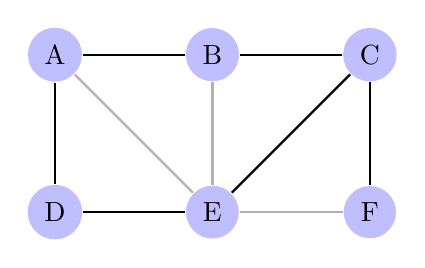
\begin{tikzpicture}
[auto,thick,node distance=2cm,every node/.style={circle,fill=blue!25}]
	\node (D) {D};
  \node (A) [above of=D] {A};
  \node (E) [right of=D] {E};
  \node (B) [right of=A] {B};
  \node (F) [right of=E] {F};
  \node (C) [right of=B] {C};

	\path
	(F) edge (C) (C) edge (B) (B) edge (A) (A) edge (D) (D) edge (E) (E) edge (C);

	\path[black!30]
	(E) edge (A)
	    edge (B)
	(F) edge (E);
\end{tikzpicture}

     \caption{Et eksempel på en vej i en simpel graf.}
     \label{graf_ikke_kreds}
   \end{minipage}
\end{figure}

\section{Sammenhængende grafer}
For en graf kan det være relevant at afgøre, om der er en vej mellem alle knuder i grafen, således, at det er muligt at komme fra en hvilken som helst knude til en anden.
I dette kapitel vil der kun blive fokuseret på ikke-orienterede grafer.

\begin{defn}
\label{def_iosmh}
En graf siges at være \textit{sammenhængende}, hvis der er en vej mellem hvert knudepar i grafen. 
\end{defn}


\begin{thm}
Der er en simpel vej mellem ethvert knudepar i en sammenhængende graf.
\label{smh_satning}
\end{thm}

\begin{proof}
Lad knuderne $u$ og $v$ være to knuder i den sammenhængende graf $G=(V,E)$.
Per Definition \ref{def_iosmh} er der en vej mellem $u$ og $v$.
Lad en kortest mulig vej mellem $u$ og $v$ være $v_0,v_1,...,v_n$, hvor $v_0=u$ og $v_n=v$.

For modstrid antages det, at denne vej ikke er simpel. 
Så er $v_i=v_j$ for $0 \leq i < j$, fordi vejen går gennem kanten $v_i,v_{i+1}$ to gange, specielt besøges $v_i$ to gange.
Det betyder, at der er en kortere vej fra $u$ til $v$, med knudesekvens $v_0,v_1,...,v_{i-1},v_j,...,v_n$, som opnåes ved at fjerne kanterne i sekvensen $v_i,...,v_{j-1}$.
Dette er i modstrid med antagelsen om, at vejen var kortest mulig.
Det må derfor gælde, at der er en simpel vej mellem alle knudepar i en sammenhængende graf. 
\end{proof}

\section{Vægtede grafer}

Flere problemstillinger kan modelleres ved brug af grafer med vægte tildelt kanterne. 
Det kan f.eks. være distance, den samlede rejsetid, eller billetprisen for at rejse mellem to byer. 
Grafer, der har vægte tildelt kanterne, kaldes vægtede grafer. 
Der opstår jævnligt forskellige typer af problemer, der involverer vægtede grafer, hvor en korteste rute, mellem to knuder i et netværk, skal bestemmes. 
Længden af en vej i en graf uden vægte er tidligere betegnet ved antallet af kanter, vejen går igennem.
I en vægtet graf er længden af vejen summen af alle kanternes vægte, der indgår i vejen. \\
I Figur \ref{fig:weighted_graph} ses et eksempel på en vægtet graf. Den kortest mulige vej fra $A$ til $D$ må være $\lbrace A,C \rbrace$, $\lbrace C,E \rbrace$, $\lbrace E,F \rbrace$, $\lbrace F,D \rbrace$. Denne vej har en længde på $5+5+5+5=20$. 

\begin{figure}[!h]
  \centering
  \begin{tikzpicture}
  [shorten >=1pt,node distance=3.1cm,on grid,auto]
    \tikzstyle{state}=[shape=circle,fill=blue!25,thick,minimum size=0.7cm]

    \node[state] (A) {$A$};
    \node[state,above of=A] (B) {$B$};
    \node[state,right of=A] (C) {$C$};
    \node[state,right of=B] (D) {$D$};
    \node[state,right of=C] (E) {$E$};
    \node[state,right of=D] (F) {$F$};

    \path[-,draw,thick]
    (A) edge node {$20$} (B)
    (A) edge node {$5$} (C)
    (B) edge node {$20$} (C)
    (B) edge node {$15$} (D)
    (C) edge node {$20$} (D)
    (C) edge node {$5$} (E)
    (D) edge node {$15$} (E)
    (D) edge node {$5$} (F)
    (E) edge node {$5$} (F)
    ;
  \end{tikzpicture}
  \caption{Eksempel på en vægtet graf.}
  \label{fig:weighted_graph}
\end{figure}

Et interessant problem, som involverer vægtede grafer, søger en kreds af kortest mulig totallængde, der besøger hver knude i en komplet graf præcis én gang. \\
I Figur \ref{fig:weighted_graph} vil en kreds af kortest mulig længde være $\lbrace A,C \rbrace$, $\lbrace C,E \rbrace$, $\lbrace E,F \rbrace$, $\lbrace F,D \rbrace$, $\lbrace D,B \rbrace$, $\lbrace B,A \rbrace$. Denne kreds har en længde på $5+5+5+5+15+20=55$. \\
Der er her tale om et eksempel på \emph{traveling salesperson problem}, som søger dén rækkefølge, knuderne skal besøges i, som resulterer i en kreds af kortest mulig længde. 
Dette problem vil projektet undersøge nærmere i et senere kapitel.

\subsection{En korteste-vej algoritme}
Der er flere algoritmer, som finder den korteste vej mellem to knuder i en vægtet graf.
Et eksempel på en sådan algoritme er Dijkstras algoritme.
Algoritmen bruges til at finde den korteste vej fra $a$ til $z$ (eller en hvilken som helst anden knude) for ikke-orienterede vægtede grafer, hvor alle vægte er positive, og kan let tilpasses orienterede grafer også. \\
Algoritmen bygger på en serie af gentagelser, hvor et sæt af knuder konstrueres, ved at tilføje én knude ved hver gentagelse. 
En knude $w$ bliver tildelt værdien (længden) af den korteste vej fra $a$ til $w$, der kun indeholder de knuder, der allerede er i sættet. 
Den knude, der tilføjes sættet, har den mindste værdi af de knuder, der allerede er en del af sættet. \\
Dijkstras algoritme starter ved at tildele $a$ værdien $0$ og de andre knuder med $\infty$. 
Der bruges notationerne $L_0(a)=0$ og $L_0(v)= \infty$ for disse, hvor $0$’et angiver, at det er den $0$te gentagelse. 
Disse værdier angiver længden af den korteste vej fra $a$ til de givne knuder, hvor vejen kun indeholder $a$. 
Der findes ingen vej fra $a$ til en knude forskellig fra $a$, hvorfor $\infty$ er længden af den korteste vej fra $a$ til en sådan knude. \\
Algoritmen fortsætter ved at forme et sæt af knuder. Sættet betegnes $S_k$ efter $k$ gentagelser. 
Til at begynde med er $S_0=\emptyset$. 
Sættet $S_k$ laves fra $S_(k-1)$ ved at tilføje en knude $u$ (med den mindste værdi), som ikke er i $S_(k-1)$.
Herefter opdateres værdierne af alle knuder, som ikke er i $S_k$, således $L_k(v)$ er længden af den korteste vej fra $a$ til $v$, som kun indeholder knuder i $S_k$. 
Den måde, hvorpå algoritmen vælger en knude $u$, der tilføjes $S_k$ ved hver gentagelse, er det optimale valg af knude, hvilket gør den til en grådig algoritme. 
Proceduren fortsætter med at tilføje knuder til sættet, indtil $z$ også er tilføjet.
Herefter tildeles $z$ den værdi, der svarer til længden af den korteste vej fra $a$ til $z$. \\
Dijkstras algoritme ses i Algoritme \ref{dijkstras_algorithm}. \\

\begin{algorithm}[!h]
\caption{Dijkstras algoritme}
\label{dijkstras_algorithm}
\textbf{procedure} $Dijkstra(G:$ vægtet sammenhængende simpel graf, med positive vægte) \\ 
$\lbrace G$ har knuder $a=v_0, v_1, \dotsc , v_n=z$ og længder $w(v_i,v_j)$ hvor $w(v_i,v_j)= \infty $ hvis $ \lbrace v_i,v_j \rbrace $ ikke er en kant i $G \rbrace$ \\
\textbf{for} $i:=1$ \textbf{til} $n$ \\
$\-$ $\-$ $\-$ $\-$ $\-$ $\-$
$L(v_i):= \infty$ \\
$L(a):=0$ \\
$S:=\emptyset$ \\
{værdien er nu fastsat, så værdien af $a$ er $0$ og alle andre værdier er $\infty$, og $S$ er et tomt sæt} \\
$\-$ $\-$ $\-$ $\-$ $\-$ $\-$
\textbf{så længe} $z \not\in S$ \\
$\-$ $\-$ $\-$ $\-$ $\-$ $\-$
$u:=a$ en knude $\not\in S$ med $L(u)$ minimum \\
$\-$ $\-$ $\-$ $\-$ $\-$ $\-$
$S:_S\cup \lbrace u \rbrace$ \\
$\-$ $\-$ $\-$ $\-$ $\-$ $\-$
\textbf{for} alle knuder $v \not\in S$ \\
$\-$ $\-$ $\-$ $\-$ $\-$ $\-$
$\-$ $\-$ $\-$ $\-$ $\-$ $\-$
\textbf{hvis} $L(u)+w(u,v)<L(v)$ \textbf{så} $L(v):=L(u)+w(u,v)$ \\
$\-$ $\-$ $\-$ $\-$ $\-$ $\-$
$\-$ $\-$ $\-$ $\-$ $\-$ $\-$
{dette tilføjer en knude til $S$ med minimal værdi og opdaterer værdien af knuderne $\not\in S$} \\
\textbf{returner} $L(z)$ {$L(z)=$ længden af den korteste vej fra $a$ til $z$}
\end{algorithm} 

Til at opsummere dette opstilles Sætning \ref{dijkstras_theorem}.
\begin{thm}\label{dijkstras_theorem}
Dijkstras algoritme finder længden af en korteste vej mellem to knuder i en sammenhængende, simpel, ikke-orienteret vægtet graf.
\end{thm}

Sætning \ref{dijkstras_theorem} kan bevises ved et induktionsbevis.

\begin{proof}
Den induktive hypotese gælder for den $k$te gentagelse. 
Lad $v$ være knuden tilføjet til $S$ ved den $(k+1)$te gentagelse, så $v$ er en knude $\not\in$ $S$ i slutningen af den $k$te gentagelse med den mindste værdi (hvis der er flere knuder af samme værdi, vælges blot én af disse). \\
Fra den induktive hypotese ses der, at knuderne i $S$ før den $(k+1)$te gentagelse er angivet med længden af den korteste vej fra $a$. 
Så er $v$ angivet med længden af den korteste vej fra $v$ til $a$. 
Hvis det ikke var tilfældet i slutningen af den $k$te gentagelse, ville der være en vej kortere end $L_k(v)$, der indeholder en knude $\not\in$ $S$. 
Lad $u$ være den første knude $\not\in$ $S$ i sådan en vej. 
Der er en vej med længder kortere end $L_k(v)$ fra $a$ til $u$ kun indeholdende knuder i $S$. 
Dette modsiger valget af $v$, da $(i)$ holdes i slutningen af den $(k+1)$te gentagelse.
Lad $u$ være en knude $\not\in$ $S$ efter $k+1$ gentagelser. 
En korteste vej fra $a$ til $u$, som kun indeholder elementer i $S$, indeholder enten $v$ eller ikke. 
Hvis den ikke indeholder $v$, er længden $L_k(u)$ ved den induktive hypotese. 
Hvis den derimod indeholder $v$, må der laves en vej fra $a$ til $v$ af kortest mulig længde, der indeholder alle elementerne i $S$ undtagen $v$, efterfulgt af kanten fra $v$ til $u$. I det tilfælde, vil længden være $L_k(v)+w(v,u)$. Dette viser, at $(ii)$ er sand, da $L_(k+1)(u)=min \lbrace L_k(u), L_k(v)+w(v,u) \rbrace$. 
\end{proof}

\section{Eulerkredse}

En bestemt type af kredse gennemgår alle kanter i en graf og kaldes Eulerkredse. 

\begin{defn}\label{euler_def}
En Eulerkreds er en simpel kreds i grafen $G$ som indeholder hver kant i $G$.
En Eulervej er en simpel vej i grafen $G$, som indeholder hver kant i $G$.  
\end{defn}
\begin{exmp}
Eksempler på en Eulerkreds og en Eulervejkan ses her: 
\end{exmp}

\begin{figure}[h]
\centering
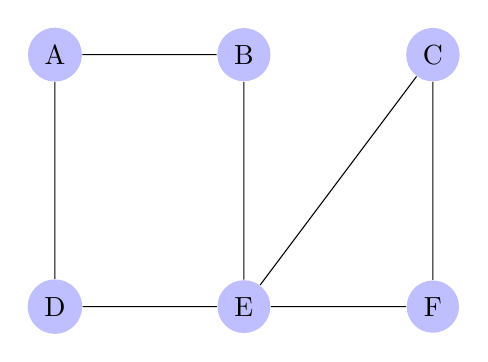
\begin{tikzpicture}
[scale=.8,auto=left,every node/.style={circle,fill=blue!25}]
  \node (n6) at (3,2) {D};
  \node (n4) at (3,6) {A};
  \node (n5) at (6,2) {E};
  \node (n1) at (6,6) {B};
  \node (n2) at (9,2) {F};
  \node (n3) at (9,6) {C};
  \foreach \from/\to in {n6/n4,n5/n1,n2/n5,n2/n3,n1/n4,n6/n5,n5/n3}
    \draw (\from) -- (\to);
\end{tikzpicture}
\caption{Euler kreds} 
\label{euler_kreds}
\end{figure}

\noindent Et eksempel på en Eulerkreds i Figur \ref{euler_kreds} kan være: $A,B,E,C,F,E,D,A$


\input{fig/tikz/euler_vej}

\noindent Et eksempel på en Eulervej i Figur \ref{euler_vej} kan være: $A,B,E,D,A,E,F,C$

\noindent Der eksiserer ikke en Eulerkreds i alle grafer. \\

For at der kan eksisere en Eulerkreds i en sammenhægende multigraf skal Sætning \ref{Eulerkreds_multigraf} gælde. 

\begin{thm}\label{Eulerkreds_multigraf}
En sammenhængende multigraf med mindst to knuder, har en Eulerkreds hvis og kun hvis, hver knude er af lige grad.
\end{thm}

\begin{proof} 
En kreds begynder i en knude $a$ og fortsætter langs en kant, som er incident med $a$, til en ny knude $b$. 
Denne kant kaldes $\lbrace a,b \rbrace$, kanten bidrager med 1 til $deg(a)$. 
Hver gang kredsen passere gennem en knude, tilføjes 2 til graden af denne knude. 
Til sidst ender kredsen tilbage i $a$, og bidrager igen med 1 til $deg(a)$. 
Derfor må $deg(a)$ være lige og graden af hver knude må også være lige.  
\end{proof} 

\noindent Det er muligt at lave en algoritme som kan finde en Eulerkreds i en multigraf.
En sådan algoritme vil første tage udgangspunkt i en tilfældig underkreds i graf G, hvorefter der indeføres en variabel H, som er lig med G, foruden kanterne i den tilfældige underkreds. 
Så længe H indeholder kanter, vil en løkke køre. 
Under denne løkke dannes en ny delkreds i H, hvor en af knuderne også skal være endepunkt for en kant i en tidligere underkreds.
Dernæst fjerns kanterne i underkredsen fra H sammen med enventuelt isolerede knuder. 
Til sidst sammensættes underkredsene til en samlet kreds, som retuneres.
Proceduren kan ses i Algoritme \ref{algoritme_euler}.
Der findes også andre algoritmer, som kan finde Eulerkredse i en graf, men disse bliver ikke nævnt i dette projekt.\\
  

\begin{algorithm}
\caption{Eulerkredse}
\label{algoritme_euler}
\textbf{procedure} Euler(G: sammenhængende mulitgraf med knuder af lige grad)\\
$kreds:=$ en kreds i G begynder i en vilkårlig knude med kanter, der danner en kreds.\\
$H:= G$ med kanterne fra $kreds$ fjernet\\
\textbf{når} $H$ har kanter\\
$\-$ $\-$ $\-$ $\-$ $\-$ $\-$
$underkreds:=$ en kreds i $H$, der begynder i en knude i $H$, som også er et endepunkt af en kant i $kreds$ \\ 
$\-$ $\-$ $\-$ $\-$ $\-$ $\-$
$H:=$ $H$ uden kanterne af $underkreds$ samt alle isolerede knuder fjernet \\
$\-$ $\-$ $\-$ $\-$ $\-$ $\-$
$kreds:=$ $kreds$ med $underkreds$ indsat ved den passende knude \\ 
\textbf{retuner} $kreds$ ($kreds$ er en Eulerkreds)
\end{algorithm}

$\-$ $\-$ $\-$ $\-$ $\-$ $\-$ \\
\noindent Hvis der ikke findes en Eulerkreds i en graf, kan der godt eksistere en Eulervej. 
For at der kan findes en Eulervej skal Sætning \ref{Eulervej_multigraf} gælde. 

\begin{thm} \label{Eulervej_multigraf}
En sammenhængende multigraf graf G har en Eulervej, men ikke en Eulerkreds, hvis og kun hvis den har præcist to knuder af ulige grad.  
\end{thm} 

\begin{proof}
Antag at en sammenhængende multigraf G har en Eulervej fra $a$ til $b$, men ikke en Eulerkreds. 
Den første kant som passeres på vejen bidrager med 1 til $deg(a)$. 
Hver gang vejen passerer knuden $a$ vil 2 tilføjes til $deg(a)$. 
Den sidste kant på vejen bidrager 1 til graden af endepunktet for vejen, $deg(b)$. 
Ligesom for $a$, kan vejen krydse $b$. 
Hver gang dette måtte ske tilføjes 2 til graden af $b$. 
Resultatet bliver, at $a$ og $b$ altid vil være af ulige grad. 
Alle andre knuder på vejen vil være af lige grad, fordi at 2 tilføjes til graden af en knude, hver gang en knude passeres.  
\end{proof}


